% ─── Slide: Final results ─────────────────────────────────────────────────────
\begin{frame}[shrink=20]{Final Results: INT4 + LoRA Surpasses INT8 PTQ}
  \begin{columns}[T]
    \begin{column}{0.52\textwidth}
      \begin{center}
      \renewcommand{\arraystretch}{1.25}
      \small
      \begin{tabular}{lccc}
        \toprule
        \textbf{Method} & \textbf{Bits} & \textbf{Wiki2} & \textbf{C4} \\
        \midrule
        FP baseline       & —    & $\sim$10.5 & $\sim$20.0 \\
        \midrule
        INT8 baseline     & w8a8 & 28.86 & — \\
        INT8 prop+center  & w8a8 & \better{14.41} & — \\
        \midrule
        INT4 pure PTQ best & w4a4 & 27.56 & — \\
        INT4 staged PTQ   & w4a4 & 27.60 & 46.40 \\
        \midrule
        \textbf{INT4 + LoRA} & \textbf{w4a4} & \best{13.96} & \best{23.30} \\
        \bottomrule
      \end{tabular}
      \end{center}

      \vspace{0.15em}
      \begin{exampleblock}{Key messages}
        \begin{itemize}
          \item \textbf{INT4 + LoRA surpasses best INT8 PTQ on WikiText2}
                (13.96 vs.\ 14.41)
          \item \textbf{Generalises to C4} ($-50\%$ vs.\ INT4 PTQ baseline):
                correction is not overfit to calibration domain
          \item CE+KL with all 7 projections is the winning config
        \end{itemize}
      \end{exampleblock}
    \end{column}
    \begin{column}{0.44\textwidth}
      % plot_final_results_wiki_c4.pdf
      \iftrue
        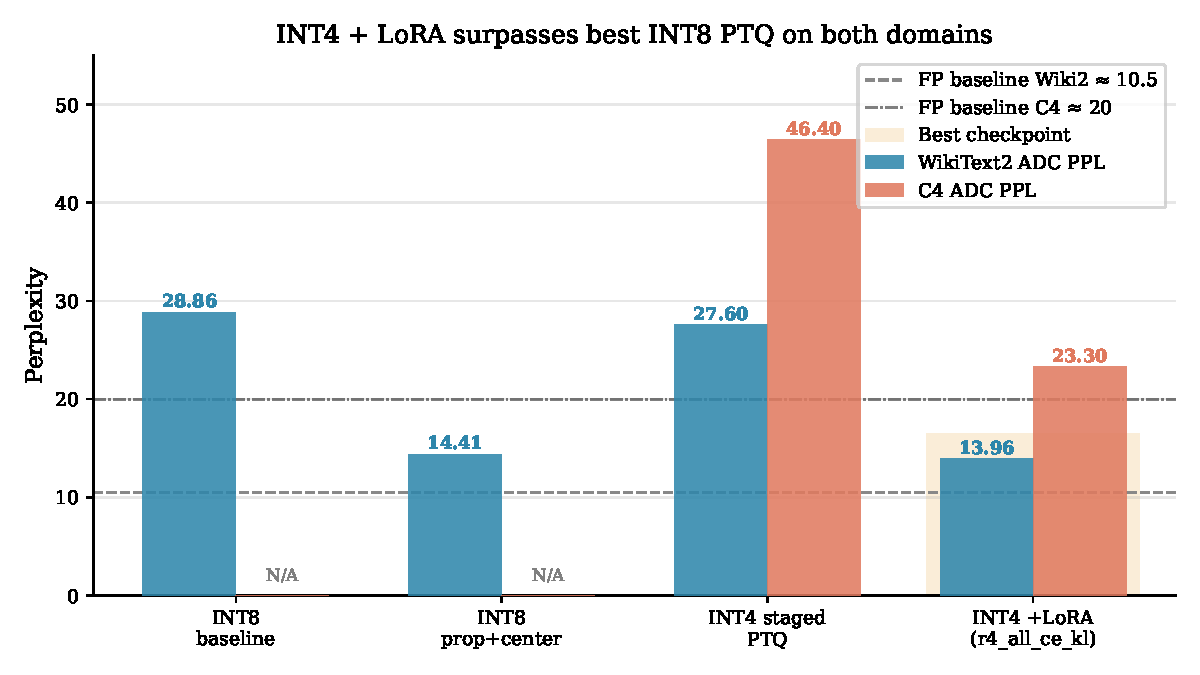
\includegraphics[width=\linewidth]{figs/plot_final_results_wiki_c4.pdf}
      \else
        \figplaceholder[0.68\textheight]{Grouped bar chart (5 methods on x-axis).
          Two bars per group: Wiki2 ADC PPL (blue) and C4 ADC PPL (orange).
          Dashed lines: FP Wiki2 $\approx$ 10.5, FP C4 $\approx$ 20.
          Highlight INT4+LoRA as the ``winner'' bar.
          Show that C4 improvement is proportionally as large as Wiki2.}
      \fi
    \end{column}
  \end{columns}
\end{frame}
